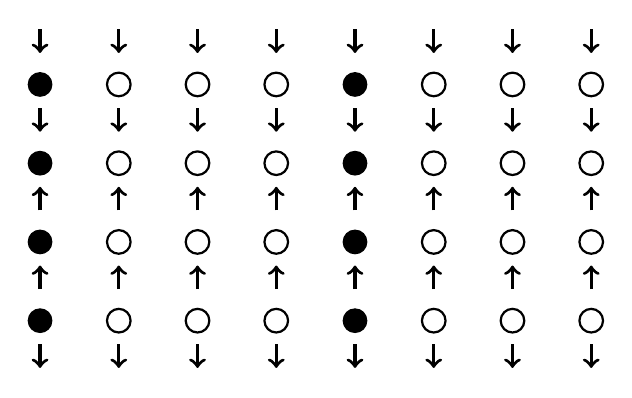
\begin{tikzpicture}
    % charge stripe
    \foreach \y in {0,1,2,3} {
        \foreach \x in {0,4} {
            \filldraw (\x+0,\y) circle [radius=0.15];
            % afm
            \draw [thick] (\x+1,\y) circle [radius=0.15];
            \draw [thick] (\x+2,\y) circle [radius=0.15];
            \draw [thick] (\x+3,\y) circle [radius=0.15];
        }
    }
    
    \foreach \x in {0,1,2,3,4,5,6,7} {
        \draw [very thick, <-] (\x,-0.6) -- (\x,-0.3);
        \draw [very thick, ->] (\x,-0.6+1) -- (\x,-0.3+1);
        \draw [very thick, ->] (\x,-0.6+2) -- (\x,-0.3+2);
        \draw [very thick, <-] (\x,-0.6+3) -- (\x,-0.3+3);
        \draw [very thick, <-] (\x,-0.6+4) -- (\x,-0.3+4);
    }
\end{tikzpicture}